\documentclass{standalone}

\usepackage[OT1]{fontenc}
\renewcommand*\familydefault{\sfdefault}
\usepackage{helvet,sfmath}
\usepackage{siunitx}

\usepackage{tikz}
\usetikzlibrary{arrows,calc,patterns}
\usepackage{tikz,tkz-euclide}


\definecolor{BlueDefault}{rgb}{0.2,0.2,0.7}

\begin{document}

\begin{tikzpicture}[scale=0.8]
    \draw[thick, fill=lightgray!20] (-2,-1) to (-1,1) to (2,1) to (1,-1) to (-2,-1);
    \draw[-Stealth] (-1,1) to (-1.5,0);
    \draw[-Stealth] (2,1) to (0.5,1);
    \draw[-Stealth] (1,-1) to (1.5,0);
    \draw[-Stealth] (-2,-1) to (-0.5,-1);

    \draw[dashed] 
    (-2,-1) to (-2.5,-2)
    (1,-1) to (0.5,-2)
    (1,-1) to (2,-1)
    (2,1) to (3,1)
    ;

    \draw[Stealth-Stealth] (-2.5,-2) to (0.5,-2);
    \draw[Stealth-Stealth] (2,-1) to (3,1);
    
    \draw 
    (0.5,0.3) node{\(S\)}
    (0,-0.7) node{\(I\)}
    (-1,-2) node[below]{\(l_1\)}
    (2.5,0) node[right]{\(l_2\)}
    (-0.5,-1) node[below]{\(1\)}
    (1.5,0) node[right]{\(2\)}
    (0.5,1) node[above]{\(3\)}
    (-1.5,0) node[left]{\(4\)}
    ;

    \draw[-Stealth] (0,0) to (-3,4);
    \draw[fill=black] (0,0) circle (0.05);
    \draw (-0.3,-0.3) node{\(O\)};
    \draw (-2,3) node{\(\mathbf{r}\)};

    \draw (1.1,3.0) node{ 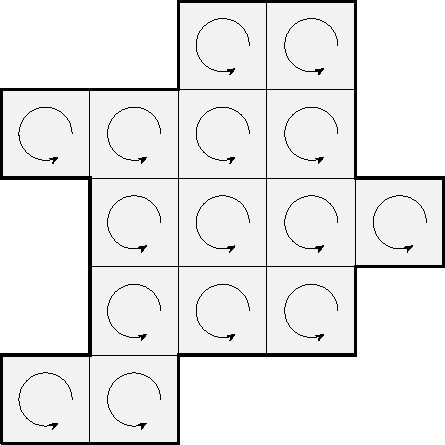
\includegraphics[width=60pt]{Figures/Magnetic_dipole_loop.pdf} };
\end{tikzpicture}    

\end{document}